%%=============================================================================
%% Inleiding
%%=============================================================================

\chapter{\IfLanguageName{dutch}{Inleiding}{Introduction}}
\label{ch:inleiding}

IT-bedrijven willen hun klanten steeds sneller te hulp kunnen schieten en betere software leveren. Vandaag de dag worstelen ze nog te vaak met deadlines die verstrijken en krijgen ze te maken met problemen tijdens de oplevering van software. Gelukkig is er doorheen de jaren al veel vooruitgang gemaakt door het toepassen van principes zoals Agile en DevOps. Agile leidt tot een betere samenwerking tussen business en IT. DevOps gaat dan weer een stapje verder. Het past een mindset toe om de samenwerking tussen alle afdelingen binnen een IT-bedrijf vlotter te laten verlopen. \\
Een Continuous Integration en Continuous Delivery (CI/CD) pipeline opzetten is een vast onderdeel van DevOps en kan de werking van een bedrijf ten goede komen. Continuous Integration wordt in gang gezet wanneer code naar de 'Source Control Repository' wordt gepusht en deze automatisch wordt getest. De Continuous Integration tool kijkt of deze voldoet aan alle kwaliteitseisen en nadien wordt er feedback gegeven over de kwaliteit van de toegevoegde code.\\
Bij Continuous Delivery wordt de build van de Continuous Integration nogmaals getest op kwaliteit. Er wordt gekeken of deze voldoet om naar Quality te brengen. Een CI/CD pipeline zorgt voor de automatisatie van testen, builds en deployment en heeft als grote voordelen het sneller doorvoeren van wijzigingen en het minimaliseren van 'downtime' van de applicatie.

Uit onderzoek - uitgevoerd door DZone - blijkt dat DevOps steeds meer ingeburgerd raakt in de bedrijfscultuur ~\autocite{Baker2019}. In 2019 werkte 48\% van de ondervraagden binnen een Operations team mee aan een Continuous Delivery pipeline, een stijging van 7\% in vergelijking met 2018.
De stijging is te danken aan het management, dat meer gelooft in de mindset van DevOps. Van de 527 ondervraagde technologiespecialisten heeft 54\% van hen de steun van het management als het gaat over DevOps. Dit wil zeggen dat we op de goede weg zijn, maar er nog werk aan de winkel is.
Als we verder naar het onderzoek kijken, blijkt dat er een duidelijk verschil is tussen de implementatie van DevOps en een CI/CD pipeline. 
Bij 31\% is er een Continuous Integration pipeline aanwezig in elk project, terwijl 33\% zegt een CI pipeline te gebruiken in enkele projecten.
Slechts 14\% van de ondervraagden bevestigt dat ze een Continuous Delivery pipeline hebben voor elk project, dat is zelfs een daling ten opzichte van 2018.
28\% gebruikt voor een aantal projecten een Continuous Delivery pipeline.

Hieruit kan men besluiten dat CI meer ingeburgerd is dan CD. In 58\% van de gevallen vloeien Continuous Integration processen niet door naar Continuous Delivery. De belangrijkste redenen voor deze 'gap' zijn de moeilijkheid van de configuration setup, de moeilijkheden van user acceptance testing (de laatste fase binnen software testing waarbij echte gebruikers de software testen) en het automatiseren van die testen.\\
Volgens 47\% van de 527 technologiespecialisten is dit te wijten aan de bedrijfscultuur die niet klaar is om Continuous Delivery toe te passen, in 2018 was dit nog 45\%.

Zoals te zien is op figuur\ref{img-survey-cicd} is er nog heel wat werk aan de winkel, maar is er toch al verbetering vastgesteld ten opzichte van vorige jaren. Dit bewijst ook dat een CI/CD pipeline en DevOps in het algemeen niet zo makkelijk op te zetten zijn. Technologisch is het vandaag niet zo bijster moeilijk om een pipeline op te zetten. Maar het veranderen van de mindset binnen een bedrijf, daar knelt vaak het schoentje.\\
Deze studie gaat echter niet al te diep in op het toepassen van de DevOps cultuur binnen een bedrijf, maar zal vooral het technische luik onder de loep nemen. Het bedrijf Amista zou graag een gepersonaliseerde vergelijking en handleiding hebben hoe een CI/CD pipeline op te starten.

\begin{figure}	
    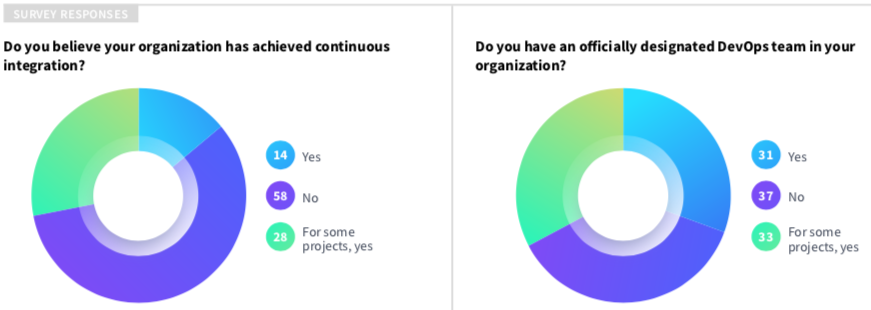
\includegraphics[scale=0.5]{survey-DZone-cicd}
    \caption{Deel van DZone's survey ~\autocite{Baker2019}} \label{img-survey-cicd}
\end{figure}

Amista is een groeiend bedrijf binnen IT consultancy. Het is een dochterbedrijf van Boutique dat zich toespitst op SAP. Amista bestaat nog maar 5 jaar en ze hebben al 60 personen in dienst. Ze mogen Infrabel, Alcopa, Danone, AG Real Estate en nog enkele andere grote merken tot hun cliënteel rekenen, zoals ook op hun site te lezen valt\footnote{https://www.amista.be}. %Algemene websites van organisaties, sofwarepakkerren, enz. mogen niet in bib file, maar als voetnoot gebruikt worden!
Ze zijn in twee landen actief, Frankrijk en België, maar werken ook samen met mensen uit India.
Amista heeft zich verdiept in Sales, Marketing en Service Management binnen bedrijven. Ze helpen hun klanten op gebied van Innovation, Integration en Digital Learning.
De missie van Amista is om samen met hun klanten, innovatieve en kwalitatieve oplossingen aan te bieden met behulp van het volledige gamma dat SAP te bieden heeft.
Amista wil graag de wensen van hun klanten zo goed mogelijk proberen te vervullen, daarom proberen ze zelf innovatief uit de hoek te komen. Ze spelen met het idee om een CI/CD pipeline op te zetten voor software development om zo hun klanten een nog betere service aan te bieden.

Om een Continuous Integration en Continuous Delivery pipeline op te stellen zijn er vandaag veel tools beschikbaar.
Deze bachelorproef zal verschillende build schedulers vergelijken op basis van de samenwerking met SAPUI5, SAP Cloud Platform, Git en Bitbucket. Er wordt vergeleken of de build scheduler past binnen een CI/CD pipeline, automated tests via Karma kan uitvoeren en bovendien wordt er gekeken naar gebruiksgemak en security.
Aan de hand van de 'winnende' build scheduler wordt er een handleiding beschreven om een pipeline op te zetten binnen een SAPUI5 webapplicatie dat verbonden is met SAP HANA en gehost wordt op SAP Cloud Platform.

\section{\IfLanguageName{dutch}{Probleemstelling}{Problem Statement}}
\label{sec:probleemstelling}
Amista heeft enkele klanten waar ze SAPUI5 webapplicaties voor maken in combinatie met een SAP HANA database die gebruik maakt van Node.js en wordt gehost op SAP Cloud Platform.
Elk bedrijf wil het beste voor zijn klanten. Voor een software consultancy bedrijf, zoals Amista, staat de service en het project dat de klant voor ogen heeft centraal en zullen ze er alles aan doen om de noden en wensen van hun klanten te vervullen.\\
Bij de oplevering van een project loopt het vaak mis: de deadline wordt vaak overschreden, wat stress en problemen met zich meebrengt. Het gebeurt vaak dat de klant een wijziging wil doorvoeren, wat de scope en planning in de war stuurt. Deze scenario's kunnen vermeden worden door een Continuous Integration en Continuous Delivery pipeline te gebruiken. Dankzij een CI/CD pipeline kan het development team sneller wijzigingen doorvoeren en krijgen ze sneller feedback van de klant. Aan de hand van een voorbeeld wordt bovenstaande verduidelijkt.

Amista heeft Appel als klant. Deze klant had in het verleden moeilijkheden met het opleveren van nieuwe projecten en wijzigen van bestaande projecten. Daarom besloten ze om een policy toe te passen waarbij de opleveringsdata gebundeld werden en om de twee weken een release-dag werd voorzien. Dit maakt het niet mogelijk om een wijziging door te voeren tussen twee datums van oplevering. Er moet telkens gewacht worden tot de volgende opleverdatum om een verandering door te voeren.\\
Appel is een internationale speler binnen zijn industrie en heeft vestigingen over heel de wereld. In één van de landen is het verplicht dat grote bedrijven de belastingen online invullen. Wanneer dit niet gebeurt hangt het bedrijf grote boetes boven het hoofd. De overheid voorziet een speciaal certificaat voor het invullen van de belastingen. De tool voor de belastingaangifte werd gehost op SAP Cloud Platform, waar Amista verantwoordelijk voor is. Een tijdje geleden werd het certificaat vernieuwd op SAP Cloud Platform tijdens een release-dag, maar de build loopt mis. Er falen verschillende processen en de applicatie loopt vast. Ze zoeken het probleem en vinden dat er een parameter in de backend moet vernieuwd worden. Hier was Amista echter niet verantwoordelijk voor en wist bijgevolg ook niet van het bestaan van deze parameter. Gezien de policy van Appel -dat er om de twee weken een release van de wijzigingen mag doorgevoerd worden- is het bedrijf niet voorbereid op onverwachte problemen. Uiteindelijk hebben ze met veel moeite iemand kunnen bereiken die de parameter in de backend kon aanpassen en kon zorgen voor een nieuwe release. Zo kon, gepaard met heel veel stress, vermeden worden dat Appel een boete kreeg.\\
Met een Continuous Integration en Continuous Delivery pipeline zou dit euvel in no-time opgelost kunnen worden. Met voldoende en goede testen zou de pipeline aangegeven hebben dat er een probleem was en zal de wijziging nooit productie halen.\\
(Bovenstaand voorbeeld bevat fictieve namen).

Om een CI/CD pipeline op te zetten binnen de hierboven beschreven omgeving is er nog niet veel informatie terug te vinden. Het probleem ligt hem in de combinatie van specifieke tools die gebruikt worden. Om te weten welke build scheduler het beste bij deze omgeving zou passen, moeten er specifieke zaken onderzocht en vergeleken worden. Op internet is niet veel informatie terug te vinden over welke build scheduler het best gebruikt wordt met een SAPUI5 applicatie, gehost op SAP Cloud Platform. Daarom wil Amista graag een gepersonaliseerde vergelijking en handleiding om een Continuous Integration en Continuous Delivery pipeline op te zetten, zodat ze hun klanten beter kunnen helpen.

\section{\IfLanguageName{dutch}{Onderzoeksvraag}{Research question}}
\label{sec:onderzoeksvraag}
\begin{itemize}
    \item Wat zijn de voor- en nadelen van een CI/CD pipeline in het algemeen en specifiek voor Amista?
    \item Is het mogelijk om een Continuous Integration en Continuous Delivery pipeline te implementeren voor de ontwikkeling van een SAPUI5 applicatie, gecombineerd met een SAP HANA database op SAP Cloud Platform?
    \item Welke tools moeten we gebruiken om een CI/CD pipeline te implementeren als we vergelijken op de samenwerking met SAPUI5, SAP Cloud Platform, Git en Bitbucket. Welke build scheduler past binnen een CI/CD pipeline, kan automated tests uitvoeren via Karma en is bovendien het veiligst en makkelijst in gebruik?
    \item Hoe kunnen we deze implementatie tot een succes brengen?
\end{itemize}

\section{\IfLanguageName{dutch}{Onderzoeksdoelstelling}{Research objective}}
\label{sec:onderzoeksdoelstelling}
Het hoofddoel van deze bachelorproef is een proof-of-concept uit te zetten over hoe een CI/CD pipeline te gebruiken in de dagelijkse werking van Amista.
Deze bachelorproef gaat daarnaast ook op zoek naar de beste tools om de pipeline op te bouwen, rekening houdend met de samenwerking tussen SAPUI5, SAP Cloud Platform, Git en Bitbucket. Er wordt vergeleken of de build scheduler past binnen een CI/CD pipeline, automated tests kan uitvoeren via Karma en bovendien wordt er gekeken naar gebruiksgemak en security.

\section{\IfLanguageName{dutch}{Opzet van deze bachelorproef}{Structure of this bachelor thesis}}
\label{sec:opzet-bachelorproef}
De rest van deze bachelorproef is als volgt opgebouwd:

In Hoofdstuk ~\ref{ch:ci-cd-cd} wordt er dieper ingegaan op de domeinen: Continuous Integration, Continuous Delivery, Continuous Deployment, DevOps en Automated Testing omdat deze toch een dominante rol spelen binnen deze bachelorproef.

De waaromvraag is minstens even belangrijk als de hoe-vraag. Concreet: wat zijn de voor- en nadelen van een CI/CD pipeline te integreren in het algemeen en specifiek voor Amista? Hoe ziet zo'n CI/CD pipeline eruit? Een antwoord op deze vragen is terug te vinden in Hoofdstuk ~\ref{ch:cicd-pipeline}.

SAP en de tools die in deze studie worden gebruikt, worden aan de hand van de gevonden literatuur beschreven in hoofdstuk ~\ref{ch:sap}.

In Hoofdstuk ~\ref{ch:methodologie} wordt de methodologie toegelicht en worden de gebruikte onderzoekstechnieken besproken om een antwoord te kunnen formuleren op de onderzoeksvragen. Dit door in grote lijnen een vergelijking te maken tussen de build schedulers die op de markt aanwezig zijn. Ook de set-up van de omgeving wordt uitvoerig besproken.

In Hoofdstuk ~\ref{ch:proof-of-concept} wordt er een gepersonaliseerde handleiding beschreven om met de beste build scheduler een CI/CD pipeline te implementeren.

Tenslotte wordt in Hoofdstuk ~\ref{ch:conclusie} de conclusie gegeven en een antwoord geformuleerd op de onderzoeksvragen. Daarbij wordt ook een aanzet gegeven voor toekomstig onderzoek binnen dit domein.